\documentclass[11pt]{article}
	\author{Nikolay Prieto Ph.D(c)}
    \usepackage[breakable]{tcolorbox}
    \usepackage{parskip} % Stop auto-indenting (to mimic markdown behaviour)
    
    \usepackage{iftex}
    \ifPDFTeX
    	\usepackage[T1]{fontenc}
    	\usepackage{mathpazo}
    \else
    	\usepackage{fontspec}
    \fi

    % Basic figure setup, for now with no caption control since it's done
    % automatically by Pandoc (which extracts ![](path) syntax from Markdown).
    \usepackage{graphicx}
    % Maintain compatibility with old templates. Remove in nbconvert 6.0
    \let\Oldincludegraphics\includegraphics
    % Ensure that by default, figures have no caption (until we provide a
    % proper Figure object with a Caption API and a way to capture that
    % in the conversion process - todo).
    \usepackage{caption}
    \DeclareCaptionFormat{nocaption}{}
    \captionsetup{format=nocaption,aboveskip=0pt,belowskip=0pt}

    \usepackage[Export]{adjustbox} % Used to constrain images to a maximum size
    \adjustboxset{max size={0.9\linewidth}{0.9\paperheight}}
    \usepackage{float}
    \floatplacement{figure}{H} % forces figures to be placed at the correct location
    \usepackage{xcolor} % Allow colors to be defined
    \usepackage{enumerate} % Needed for markdown enumerations to work
    \usepackage{geometry} % Used to adjust the document margins
    \usepackage{amsmath} % Equations
    \usepackage{amssymb} % Equations
    \usepackage{textcomp} % defines textquotesingle
    % Hack from http://tex.stackexchange.com/a/47451/13684:
    \AtBeginDocument{%
        \def\PYZsq{\textquotesingle}% Upright quotes in Pygmentized code
    }
    \usepackage{upquote} % Upright quotes for verbatim code
    \usepackage{eurosym} % defines \euro
    \usepackage[mathletters]{ucs} % Extended unicode (utf-8) support
    \usepackage{fancyvrb} % verbatim replacement that allows latex
    \usepackage{grffile} % extends the file name processing of package graphics 
                         % to support a larger range
    \makeatletter % fix for grffile with XeLaTeX
    \def\Gread@@xetex#1{%
      \IfFileExists{"\Gin@base".bb}%
      {\Gread@eps{\Gin@base.bb}}%
      {\Gread@@xetex@aux#1}%
    }
    \makeatother

    % The hyperref package gives us a pdf with properly built
    % internal navigation ('pdf bookmarks' for the table of contents,
    % internal cross-reference links, web links for URLs, etc.)
    \usepackage{hyperref}
    % The default LaTeX title has an obnoxious amount of whitespace. By default,
    % titling removes some of it. It also provides customization options.
    \usepackage{titling}
    \usepackage{longtable} % longtable support required by pandoc >1.10
    \usepackage{booktabs}  % table support for pandoc > 1.12.2
    \usepackage[inline]{enumitem} % IRkernel/repr support (it uses the enumerate* environment)
    \usepackage[normalem]{ulem} % ulem is needed to support strikethroughs (\sout)
                                % normalem makes italics be italics, not underlines
    \usepackage{mathrsfs}
    

    
    % Colors for the hyperref package
    \definecolor{urlcolor}{rgb}{0,.145,.698}
    \definecolor{linkcolor}{rgb}{.71,0.21,0.01}
    \definecolor{citecolor}{rgb}{.12,.54,.11}

    % ANSI colors
    \definecolor{ansi-black}{HTML}{3E424D}
    \definecolor{ansi-black-intense}{HTML}{282C36}
    \definecolor{ansi-red}{HTML}{E75C58}
    \definecolor{ansi-red-intense}{HTML}{B22B31}
    \definecolor{ansi-green}{HTML}{00A250}
    \definecolor{ansi-green-intense}{HTML}{007427}
    \definecolor{ansi-yellow}{HTML}{DDB62B}
    \definecolor{ansi-yellow-intense}{HTML}{B27D12}
    \definecolor{ansi-blue}{HTML}{208FFB}
    \definecolor{ansi-blue-intense}{HTML}{0065CA}
    \definecolor{ansi-magenta}{HTML}{D160C4}
    \definecolor{ansi-magenta-intense}{HTML}{A03196}
    \definecolor{ansi-cyan}{HTML}{60C6C8}
    \definecolor{ansi-cyan-intense}{HTML}{258F8F}
    \definecolor{ansi-white}{HTML}{C5C1B4}
    \definecolor{ansi-white-intense}{HTML}{A1A6B2}
    \definecolor{ansi-default-inverse-fg}{HTML}{FFFFFF}
    \definecolor{ansi-default-inverse-bg}{HTML}{000000}

    % commands and environments needed by pandoc snippets
    % extracted from the output of `pandoc -s`
    \providecommand{\tightlist}{%
      \setlength{\itemsep}{0pt}\setlength{\parskip}{0pt}}
    \DefineVerbatimEnvironment{Highlighting}{Verbatim}{commandchars=\\\{\}}
    % Add ',fontsize=\small' for more characters per line
    \newenvironment{Shaded}{}{}
    \newcommand{\KeywordTok}[1]{\textcolor[rgb]{0.00,0.44,0.13}{\textbf{{#1}}}}
    \newcommand{\DataTypeTok}[1]{\textcolor[rgb]{0.56,0.13,0.00}{{#1}}}
    \newcommand{\DecValTok}[1]{\textcolor[rgb]{0.25,0.63,0.44}{{#1}}}
    \newcommand{\BaseNTok}[1]{\textcolor[rgb]{0.25,0.63,0.44}{{#1}}}
    \newcommand{\FloatTok}[1]{\textcolor[rgb]{0.25,0.63,0.44}{{#1}}}
    \newcommand{\CharTok}[1]{\textcolor[rgb]{0.25,0.44,0.63}{{#1}}}
    \newcommand{\StringTok}[1]{\textcolor[rgb]{0.25,0.44,0.63}{{#1}}}
    \newcommand{\CommentTok}[1]{\textcolor[rgb]{0.38,0.63,0.69}{\textit{{#1}}}}
    \newcommand{\OtherTok}[1]{\textcolor[rgb]{0.00,0.44,0.13}{{#1}}}
    \newcommand{\AlertTok}[1]{\textcolor[rgb]{1.00,0.00,0.00}{\textbf{{#1}}}}
    \newcommand{\FunctionTok}[1]{\textcolor[rgb]{0.02,0.16,0.49}{{#1}}}
    \newcommand{\RegionMarkerTok}[1]{{#1}}
    \newcommand{\ErrorTok}[1]{\textcolor[rgb]{1.00,0.00,0.00}{\textbf{{#1}}}}
    \newcommand{\NormalTok}[1]{{#1}}
    
    % Additional commands for more recent versions of Pandoc
    \newcommand{\ConstantTok}[1]{\textcolor[rgb]{0.53,0.00,0.00}{{#1}}}
    \newcommand{\SpecialCharTok}[1]{\textcolor[rgb]{0.25,0.44,0.63}{{#1}}}
    \newcommand{\VerbatimStringTok}[1]{\textcolor[rgb]{0.25,0.44,0.63}{{#1}}}
    \newcommand{\SpecialStringTok}[1]{\textcolor[rgb]{0.73,0.40,0.53}{{#1}}}
    \newcommand{\ImportTok}[1]{{#1}}
    \newcommand{\DocumentationTok}[1]{\textcolor[rgb]{0.73,0.13,0.13}{\textit{{#1}}}}
    \newcommand{\AnnotationTok}[1]{\textcolor[rgb]{0.38,0.63,0.69}{\textbf{\textit{{#1}}}}}
    \newcommand{\CommentVarTok}[1]{\textcolor[rgb]{0.38,0.63,0.69}{\textbf{\textit{{#1}}}}}
    \newcommand{\VariableTok}[1]{\textcolor[rgb]{0.10,0.09,0.49}{{#1}}}
    \newcommand{\ControlFlowTok}[1]{\textcolor[rgb]{0.00,0.44,0.13}{\textbf{{#1}}}}
    \newcommand{\OperatorTok}[1]{\textcolor[rgb]{0.40,0.40,0.40}{{#1}}}
    \newcommand{\BuiltInTok}[1]{{#1}}
    \newcommand{\ExtensionTok}[1]{{#1}}
    \newcommand{\PreprocessorTok}[1]{\textcolor[rgb]{0.74,0.48,0.00}{{#1}}}
    \newcommand{\AttributeTok}[1]{\textcolor[rgb]{0.49,0.56,0.16}{{#1}}}
    \newcommand{\InformationTok}[1]{\textcolor[rgb]{0.38,0.63,0.69}{\textbf{\textit{{#1}}}}}
    \newcommand{\WarningTok}[1]{\textcolor[rgb]{0.38,0.63,0.69}{\textbf{\textit{{#1}}}}}
    
    
    % Define a nice break command that doesn't care if a line doesn't already
    % exist.
    \def\br{\hspace*{\fill} \\* }
    % Math Jax compatibility definitions
    \def\gt{>}
    \def\lt{<}
    \let\Oldtex\TeX
    \let\Oldlatex\LaTeX
    \renewcommand{\TeX}{\textrm{\Oldtex}}
    \renewcommand{\LaTeX}{\textrm{\Oldlatex}}
    % Document parameters
    % Document title
    \title{Regression Task 2020II}
    
    
    
    
    
% Pygments definitions
\makeatletter
\def\PY@reset{\let\PY@it=\relax \let\PY@bf=\relax%
    \let\PY@ul=\relax \let\PY@tc=\relax%
    \let\PY@bc=\relax \let\PY@ff=\relax}
\def\PY@tok#1{\csname PY@tok@#1\endcsname}
\def\PY@toks#1+{\ifx\relax#1\empty\else%
    \PY@tok{#1}\expandafter\PY@toks\fi}
\def\PY@do#1{\PY@bc{\PY@tc{\PY@ul{%
    \PY@it{\PY@bf{\PY@ff{#1}}}}}}}
\def\PY#1#2{\PY@reset\PY@toks#1+\relax+\PY@do{#2}}

\expandafter\def\csname PY@tok@w\endcsname{\def\PY@tc##1{\textcolor[rgb]{0.73,0.73,0.73}{##1}}}
\expandafter\def\csname PY@tok@c\endcsname{\let\PY@it=\textit\def\PY@tc##1{\textcolor[rgb]{0.25,0.50,0.50}{##1}}}
\expandafter\def\csname PY@tok@cp\endcsname{\def\PY@tc##1{\textcolor[rgb]{0.74,0.48,0.00}{##1}}}
\expandafter\def\csname PY@tok@k\endcsname{\let\PY@bf=\textbf\def\PY@tc##1{\textcolor[rgb]{0.00,0.50,0.00}{##1}}}
\expandafter\def\csname PY@tok@kp\endcsname{\def\PY@tc##1{\textcolor[rgb]{0.00,0.50,0.00}{##1}}}
\expandafter\def\csname PY@tok@kt\endcsname{\def\PY@tc##1{\textcolor[rgb]{0.69,0.00,0.25}{##1}}}
\expandafter\def\csname PY@tok@o\endcsname{\def\PY@tc##1{\textcolor[rgb]{0.40,0.40,0.40}{##1}}}
\expandafter\def\csname PY@tok@ow\endcsname{\let\PY@bf=\textbf\def\PY@tc##1{\textcolor[rgb]{0.67,0.13,1.00}{##1}}}
\expandafter\def\csname PY@tok@nb\endcsname{\def\PY@tc##1{\textcolor[rgb]{0.00,0.50,0.00}{##1}}}
\expandafter\def\csname PY@tok@nf\endcsname{\def\PY@tc##1{\textcolor[rgb]{0.00,0.00,1.00}{##1}}}
\expandafter\def\csname PY@tok@nc\endcsname{\let\PY@bf=\textbf\def\PY@tc##1{\textcolor[rgb]{0.00,0.00,1.00}{##1}}}
\expandafter\def\csname PY@tok@nn\endcsname{\let\PY@bf=\textbf\def\PY@tc##1{\textcolor[rgb]{0.00,0.00,1.00}{##1}}}
\expandafter\def\csname PY@tok@ne\endcsname{\let\PY@bf=\textbf\def\PY@tc##1{\textcolor[rgb]{0.82,0.25,0.23}{##1}}}
\expandafter\def\csname PY@tok@nv\endcsname{\def\PY@tc##1{\textcolor[rgb]{0.10,0.09,0.49}{##1}}}
\expandafter\def\csname PY@tok@no\endcsname{\def\PY@tc##1{\textcolor[rgb]{0.53,0.00,0.00}{##1}}}
\expandafter\def\csname PY@tok@nl\endcsname{\def\PY@tc##1{\textcolor[rgb]{0.63,0.63,0.00}{##1}}}
\expandafter\def\csname PY@tok@ni\endcsname{\let\PY@bf=\textbf\def\PY@tc##1{\textcolor[rgb]{0.60,0.60,0.60}{##1}}}
\expandafter\def\csname PY@tok@na\endcsname{\def\PY@tc##1{\textcolor[rgb]{0.49,0.56,0.16}{##1}}}
\expandafter\def\csname PY@tok@nt\endcsname{\let\PY@bf=\textbf\def\PY@tc##1{\textcolor[rgb]{0.00,0.50,0.00}{##1}}}
\expandafter\def\csname PY@tok@nd\endcsname{\def\PY@tc##1{\textcolor[rgb]{0.67,0.13,1.00}{##1}}}
\expandafter\def\csname PY@tok@s\endcsname{\def\PY@tc##1{\textcolor[rgb]{0.73,0.13,0.13}{##1}}}
\expandafter\def\csname PY@tok@sd\endcsname{\let\PY@it=\textit\def\PY@tc##1{\textcolor[rgb]{0.73,0.13,0.13}{##1}}}
\expandafter\def\csname PY@tok@si\endcsname{\let\PY@bf=\textbf\def\PY@tc##1{\textcolor[rgb]{0.73,0.40,0.53}{##1}}}
\expandafter\def\csname PY@tok@se\endcsname{\let\PY@bf=\textbf\def\PY@tc##1{\textcolor[rgb]{0.73,0.40,0.13}{##1}}}
\expandafter\def\csname PY@tok@sr\endcsname{\def\PY@tc##1{\textcolor[rgb]{0.73,0.40,0.53}{##1}}}
\expandafter\def\csname PY@tok@ss\endcsname{\def\PY@tc##1{\textcolor[rgb]{0.10,0.09,0.49}{##1}}}
\expandafter\def\csname PY@tok@sx\endcsname{\def\PY@tc##1{\textcolor[rgb]{0.00,0.50,0.00}{##1}}}
\expandafter\def\csname PY@tok@m\endcsname{\def\PY@tc##1{\textcolor[rgb]{0.40,0.40,0.40}{##1}}}
\expandafter\def\csname PY@tok@gh\endcsname{\let\PY@bf=\textbf\def\PY@tc##1{\textcolor[rgb]{0.00,0.00,0.50}{##1}}}
\expandafter\def\csname PY@tok@gu\endcsname{\let\PY@bf=\textbf\def\PY@tc##1{\textcolor[rgb]{0.50,0.00,0.50}{##1}}}
\expandafter\def\csname PY@tok@gd\endcsname{\def\PY@tc##1{\textcolor[rgb]{0.63,0.00,0.00}{##1}}}
\expandafter\def\csname PY@tok@gi\endcsname{\def\PY@tc##1{\textcolor[rgb]{0.00,0.63,0.00}{##1}}}
\expandafter\def\csname PY@tok@gr\endcsname{\def\PY@tc##1{\textcolor[rgb]{1.00,0.00,0.00}{##1}}}
\expandafter\def\csname PY@tok@ge\endcsname{\let\PY@it=\textit}
\expandafter\def\csname PY@tok@gs\endcsname{\let\PY@bf=\textbf}
\expandafter\def\csname PY@tok@gp\endcsname{\let\PY@bf=\textbf\def\PY@tc##1{\textcolor[rgb]{0.00,0.00,0.50}{##1}}}
\expandafter\def\csname PY@tok@go\endcsname{\def\PY@tc##1{\textcolor[rgb]{0.53,0.53,0.53}{##1}}}
\expandafter\def\csname PY@tok@gt\endcsname{\def\PY@tc##1{\textcolor[rgb]{0.00,0.27,0.87}{##1}}}
\expandafter\def\csname PY@tok@err\endcsname{\def\PY@bc##1{\setlength{\fboxsep}{0pt}\fcolorbox[rgb]{1.00,0.00,0.00}{1,1,1}{\strut ##1}}}
\expandafter\def\csname PY@tok@kc\endcsname{\let\PY@bf=\textbf\def\PY@tc##1{\textcolor[rgb]{0.00,0.50,0.00}{##1}}}
\expandafter\def\csname PY@tok@kd\endcsname{\let\PY@bf=\textbf\def\PY@tc##1{\textcolor[rgb]{0.00,0.50,0.00}{##1}}}
\expandafter\def\csname PY@tok@kn\endcsname{\let\PY@bf=\textbf\def\PY@tc##1{\textcolor[rgb]{0.00,0.50,0.00}{##1}}}
\expandafter\def\csname PY@tok@kr\endcsname{\let\PY@bf=\textbf\def\PY@tc##1{\textcolor[rgb]{0.00,0.50,0.00}{##1}}}
\expandafter\def\csname PY@tok@bp\endcsname{\def\PY@tc##1{\textcolor[rgb]{0.00,0.50,0.00}{##1}}}
\expandafter\def\csname PY@tok@fm\endcsname{\def\PY@tc##1{\textcolor[rgb]{0.00,0.00,1.00}{##1}}}
\expandafter\def\csname PY@tok@vc\endcsname{\def\PY@tc##1{\textcolor[rgb]{0.10,0.09,0.49}{##1}}}
\expandafter\def\csname PY@tok@vg\endcsname{\def\PY@tc##1{\textcolor[rgb]{0.10,0.09,0.49}{##1}}}
\expandafter\def\csname PY@tok@vi\endcsname{\def\PY@tc##1{\textcolor[rgb]{0.10,0.09,0.49}{##1}}}
\expandafter\def\csname PY@tok@vm\endcsname{\def\PY@tc##1{\textcolor[rgb]{0.10,0.09,0.49}{##1}}}
\expandafter\def\csname PY@tok@sa\endcsname{\def\PY@tc##1{\textcolor[rgb]{0.73,0.13,0.13}{##1}}}
\expandafter\def\csname PY@tok@sb\endcsname{\def\PY@tc##1{\textcolor[rgb]{0.73,0.13,0.13}{##1}}}
\expandafter\def\csname PY@tok@sc\endcsname{\def\PY@tc##1{\textcolor[rgb]{0.73,0.13,0.13}{##1}}}
\expandafter\def\csname PY@tok@dl\endcsname{\def\PY@tc##1{\textcolor[rgb]{0.73,0.13,0.13}{##1}}}
\expandafter\def\csname PY@tok@s2\endcsname{\def\PY@tc##1{\textcolor[rgb]{0.73,0.13,0.13}{##1}}}
\expandafter\def\csname PY@tok@sh\endcsname{\def\PY@tc##1{\textcolor[rgb]{0.73,0.13,0.13}{##1}}}
\expandafter\def\csname PY@tok@s1\endcsname{\def\PY@tc##1{\textcolor[rgb]{0.73,0.13,0.13}{##1}}}
\expandafter\def\csname PY@tok@mb\endcsname{\def\PY@tc##1{\textcolor[rgb]{0.40,0.40,0.40}{##1}}}
\expandafter\def\csname PY@tok@mf\endcsname{\def\PY@tc##1{\textcolor[rgb]{0.40,0.40,0.40}{##1}}}
\expandafter\def\csname PY@tok@mh\endcsname{\def\PY@tc##1{\textcolor[rgb]{0.40,0.40,0.40}{##1}}}
\expandafter\def\csname PY@tok@mi\endcsname{\def\PY@tc##1{\textcolor[rgb]{0.40,0.40,0.40}{##1}}}
\expandafter\def\csname PY@tok@il\endcsname{\def\PY@tc##1{\textcolor[rgb]{0.40,0.40,0.40}{##1}}}
\expandafter\def\csname PY@tok@mo\endcsname{\def\PY@tc##1{\textcolor[rgb]{0.40,0.40,0.40}{##1}}}
\expandafter\def\csname PY@tok@ch\endcsname{\let\PY@it=\textit\def\PY@tc##1{\textcolor[rgb]{0.25,0.50,0.50}{##1}}}
\expandafter\def\csname PY@tok@cm\endcsname{\let\PY@it=\textit\def\PY@tc##1{\textcolor[rgb]{0.25,0.50,0.50}{##1}}}
\expandafter\def\csname PY@tok@cpf\endcsname{\let\PY@it=\textit\def\PY@tc##1{\textcolor[rgb]{0.25,0.50,0.50}{##1}}}
\expandafter\def\csname PY@tok@c1\endcsname{\let\PY@it=\textit\def\PY@tc##1{\textcolor[rgb]{0.25,0.50,0.50}{##1}}}
\expandafter\def\csname PY@tok@cs\endcsname{\let\PY@it=\textit\def\PY@tc##1{\textcolor[rgb]{0.25,0.50,0.50}{##1}}}

\def\PYZbs{\char`\\}
\def\PYZus{\char`\_}
\def\PYZob{\char`\{}
\def\PYZcb{\char`\}}
\def\PYZca{\char`\^}
\def\PYZam{\char`\&}
\def\PYZlt{\char`\<}
\def\PYZgt{\char`\>}
\def\PYZsh{\char`\#}
\def\PYZpc{\char`\%}
\def\PYZdl{\char`\$}
\def\PYZhy{\char`\-}
\def\PYZsq{\char`\'}
\def\PYZdq{\char`\"}
\def\PYZti{\char`\~}
% for compatibility with earlier versions
\def\PYZat{@}
\def\PYZlb{[}
\def\PYZrb{]}
\makeatother


    % For linebreaks inside Verbatim environment from package fancyvrb. 
    \makeatletter
        \newbox\Wrappedcontinuationbox 
        \newbox\Wrappedvisiblespacebox 
        \newcommand*\Wrappedvisiblespace {\textcolor{red}{\textvisiblespace}} 
        \newcommand*\Wrappedcontinuationsymbol {\textcolor{red}{\llap{\tiny$\m@th\hookrightarrow$}}} 
        \newcommand*\Wrappedcontinuationindent {3ex } 
        \newcommand*\Wrappedafterbreak {\kern\Wrappedcontinuationindent\copy\Wrappedcontinuationbox} 
        % Take advantage of the already applied Pygments mark-up to insert 
        % potential linebreaks for TeX processing. 
        %        {, <, #, %, $, ' and ": go to next line. 
        %        _, }, ^, &, >, - and ~: stay at end of broken line. 
        % Use of \textquotesingle for straight quote. 
        \newcommand*\Wrappedbreaksatspecials {% 
            \def\PYGZus{\discretionary{\char`\_}{\Wrappedafterbreak}{\char`\_}}% 
            \def\PYGZob{\discretionary{}{\Wrappedafterbreak\char`\{}{\char`\{}}% 
            \def\PYGZcb{\discretionary{\char`\}}{\Wrappedafterbreak}{\char`\}}}% 
            \def\PYGZca{\discretionary{\char`\^}{\Wrappedafterbreak}{\char`\^}}% 
            \def\PYGZam{\discretionary{\char`\&}{\Wrappedafterbreak}{\char`\&}}% 
            \def\PYGZlt{\discretionary{}{\Wrappedafterbreak\char`\<}{\char`\<}}% 
            \def\PYGZgt{\discretionary{\char`\>}{\Wrappedafterbreak}{\char`\>}}% 
            \def\PYGZsh{\discretionary{}{\Wrappedafterbreak\char`\#}{\char`\#}}% 
            \def\PYGZpc{\discretionary{}{\Wrappedafterbreak\char`\%}{\char`\%}}% 
            \def\PYGZdl{\discretionary{}{\Wrappedafterbreak\char`\$}{\char`\$}}% 
            \def\PYGZhy{\discretionary{\char`\-}{\Wrappedafterbreak}{\char`\-}}% 
            \def\PYGZsq{\discretionary{}{\Wrappedafterbreak\textquotesingle}{\textquotesingle}}% 
            \def\PYGZdq{\discretionary{}{\Wrappedafterbreak\char`\"}{\char`\"}}% 
            \def\PYGZti{\discretionary{\char`\~}{\Wrappedafterbreak}{\char`\~}}% 
        } 
        % Some characters . , ; ? ! / are not pygmentized. 
        % This macro makes them "active" and they will insert potential linebreaks 
        \newcommand*\Wrappedbreaksatpunct {% 
            \lccode`\~`\.\lowercase{\def~}{\discretionary{\hbox{\char`\.}}{\Wrappedafterbreak}{\hbox{\char`\.}}}% 
            \lccode`\~`\,\lowercase{\def~}{\discretionary{\hbox{\char`\,}}{\Wrappedafterbreak}{\hbox{\char`\,}}}% 
            \lccode`\~`\;\lowercase{\def~}{\discretionary{\hbox{\char`\;}}{\Wrappedafterbreak}{\hbox{\char`\;}}}% 
            \lccode`\~`\:\lowercase{\def~}{\discretionary{\hbox{\char`\:}}{\Wrappedafterbreak}{\hbox{\char`\:}}}% 
            \lccode`\~`\?\lowercase{\def~}{\discretionary{\hbox{\char`\?}}{\Wrappedafterbreak}{\hbox{\char`\?}}}% 
            \lccode`\~`\!\lowercase{\def~}{\discretionary{\hbox{\char`\!}}{\Wrappedafterbreak}{\hbox{\char`\!}}}% 
            \lccode`\~`\/\lowercase{\def~}{\discretionary{\hbox{\char`\/}}{\Wrappedafterbreak}{\hbox{\char`\/}}}% 
            \catcode`\.\active
            \catcode`\,\active 
            \catcode`\;\active
            \catcode`\:\active
            \catcode`\?\active
            \catcode`\!\active
            \catcode`\/\active 
            \lccode`\~`\~ 	
        }
    \makeatother

    \let\OriginalVerbatim=\Verbatim
    \makeatletter
    \renewcommand{\Verbatim}[1][1]{%
        %\parskip\z@skip
        \sbox\Wrappedcontinuationbox {\Wrappedcontinuationsymbol}%
        \sbox\Wrappedvisiblespacebox {\FV@SetupFont\Wrappedvisiblespace}%
        \def\FancyVerbFormatLine ##1{\hsize\linewidth
            \vtop{\raggedright\hyphenpenalty\z@\exhyphenpenalty\z@
                \doublehyphendemerits\z@\finalhyphendemerits\z@
                \strut ##1\strut}%
        }%
        % If the linebreak is at a space, the latter will be displayed as visible
        % space at end of first line, and a continuation symbol starts next line.
        % Stretch/shrink are however usually zero for typewriter font.
        \def\FV@Space {%
            \nobreak\hskip\z@ plus\fontdimen3\font minus\fontdimen4\font
            \discretionary{\copy\Wrappedvisiblespacebox}{\Wrappedafterbreak}
            {\kern\fontdimen2\font}%
        }%
        
        % Allow breaks at special characters using \PYG... macros.
        \Wrappedbreaksatspecials
        % Breaks at punctuation characters . , ; ? ! and / need catcode=\active 	
        \OriginalVerbatim[#1,codes*=\Wrappedbreaksatpunct]%
    }
    \makeatother

    % Exact colors from NB
    \definecolor{incolor}{HTML}{303F9F}
    \definecolor{outcolor}{HTML}{D84315}
    \definecolor{cellborder}{HTML}{CFCFCF}
    \definecolor{cellbackground}{HTML}{F7F7F7}
    
    % prompt
    \makeatletter
    \newcommand{\boxspacing}{\kern\kvtcb@left@rule\kern\kvtcb@boxsep}
    \makeatother
    \newcommand{\prompt}[4]{
        \ttfamily\llap{{\color{#2}[#3]:\hspace{3pt}#4}}\vspace{-\baselineskip}
    }
    

    
    % Prevent overflowing lines due to hard-to-break entities
    \sloppy 
    % Setup hyperref package
    \hypersetup{
      breaklinks=true,  % so long urls are correctly broken across lines
      colorlinks=true,
      urlcolor=urlcolor,
      linkcolor=linkcolor,
      citecolor=citecolor,
      }
    % Slightly bigger margins than the latex defaults
    
    \geometry{verbose,tmargin=1in,bmargin=1in,lmargin=1in,rmargin=1in}
    
    

\begin{document}
    
    \maketitle
    
    

    
    \hypertarget{regression-task-for-intelligence-systems}{%
\section{Regression task for Intelligence
Systems}\label{regression-task-for-intelligence-systems}}

Regression tasks in Artificial Intelligence are not common, they are
being used in fields as Finance, Surrogate Modelling
\cite{Forrester2008} and Sensitivity Analysis \cite{Iooss2015}. This
time your work will be focused in design, especifically, design of
transtibial (Ankle-foot) prosthesis.

The Design Variables in prosthesis have been studied along decades.
Those variables can be grouped in the following according to
\cite{Hansen2016}:

\begin{itemize}
\tightlist
\item
  Siffness/Flexibility.
\item
  Damping.
\item
  Roll-over characteristics
\item
  Active push-off in late stance phase
\end{itemize}

The half part of the course will do the design focused on the prosthesis
stiffness, in other words, variation of the thickness along the
laminates.The other half of the course will be focused on the Roll-over
characteristics, this is achieved with variations in the prosthesis
shape.

\hypertarget{design-for-thickness}{%
\subsection{Design for thickness}\label{design-for-thickness}}

As it was explained, there are two datasets, those are simulations
already performed with a Latin Hyper Cube (LHS) experiment
\cite{Helton2003} design. The first one is about the influence of the
thickness variation with respect to the outputs. For thickness 120
simulations were run, varying the thickness on different locations of
the prosthesis. The following figure \ref{fig:thickness} explains how
thickness is being varied along the device. In total, there are twelve
dimensions as features for the dataset.

\begin{figure}[h]
    \centering
    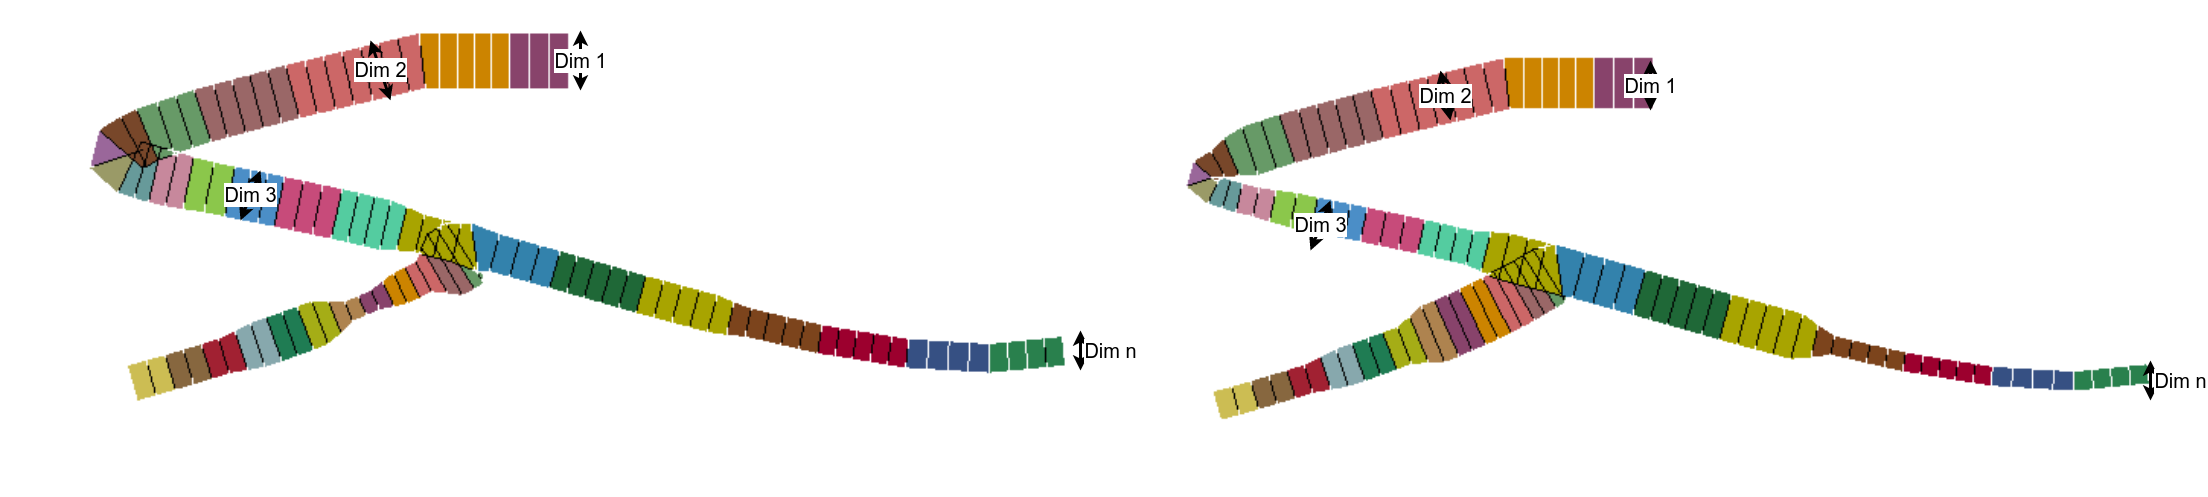
\includegraphics{Thickness_variationAF.png}
    \caption{two different samples with different thickness on each dimension, this was performed with a LHS technique.}
    \label{fig:thickness}
\end{figure}

    \begin{tcolorbox}[breakable, size=fbox, boxrule=1pt, pad at break*=1mm,colback=cellbackground, colframe=cellborder]
\prompt{In}{incolor}{6}{\boxspacing}
\begin{Verbatim}[commandchars=\\\{\}]
\PY{k+kn}{import} \PY{n+nn}{pandas} \PY{k}{as} \PY{n+nn}{pd}
\PY{n}{Thickness\PYZus{}df} \PY{o}{=} \PY{n}{pd}\PY{o}{.}\PY{n}{read\PYZus{}csv}\PY{p}{(}\PY{l+s+s1}{\PYZsq{}}\PY{l+s+s1}{AnkleFoot\PYZus{}thickness.csv}\PY{l+s+s1}{\PYZsq{}}\PY{p}{,} \PY{n}{index\PYZus{}col}\PY{o}{=}\PY{l+m+mi}{0}\PY{p}{)}
\PY{n}{Thickness\PYZus{}df}\PY{o}{.}\PY{n}{index} \PY{o}{=} \PY{n}{Thickness\PYZus{}df}\PY{p}{[}\PY{l+s+s1}{\PYZsq{}}\PY{l+s+s1}{Experiment No.}\PY{l+s+s1}{\PYZsq{}}\PY{p}{]}\PY{o}{.}\PY{n}{astype}\PY{p}{(}\PY{l+s+s1}{\PYZsq{}}\PY{l+s+s1}{int64}\PY{l+s+s1}{\PYZsq{}}\PY{p}{)} \PY{c+c1}{\PYZsh{}Establiching index experiment}
\PY{n}{Thickness\PYZus{}df\PYZus{}df} \PY{o}{=}  \PY{n}{Thickness\PYZus{}df}\PY{o}{.}\PY{n}{drop}\PY{p}{(}\PY{p}{[}\PY{l+s+s1}{\PYZsq{}}\PY{l+s+s1}{Experiment No.}\PY{l+s+s1}{\PYZsq{}}\PY{p}{]}\PY{p}{,} \PY{n}{axis}\PY{o}{=}\PY{l+m+mi}{1}\PY{p}{)} \PY{c+c1}{\PYZsh{}Dropping index column}
\PY{n}{Thickness\PYZus{}df}\PY{o}{.}\PY{n}{head}\PY{p}{(}\PY{p}{)}\PY{o}{.}\PY{n}{iloc}\PY{p}{[}\PY{p}{:}\PY{p}{,}\PY{p}{:}\PY{l+m+mi}{10}\PY{p}{]}
\end{Verbatim}
\end{tcolorbox}

            \begin{tcolorbox}[breakable, size=fbox, boxrule=.5pt, pad at break*=1mm, opacityfill=0]
\prompt{Out}{outcolor}{6}{\boxspacing}
\begin{Verbatim}[commandchars=\\\{\}]
                 dim 1   dim 2   dim 3   dim 4   dim 5   dim 6   dim 7  \textbackslash{}
Experiment No.
1               14.696  19.446   6.146   2.346   9.312  10.737  18.179
2               10.262   2.979  10.262  17.546  10.896  17.071  10.104
3               15.013   9.629  18.021   8.679   6.146  19.921  11.688
4                9.629   7.571   1.396   8.204  17.229  13.904   1.238
5                4.404   3.771  15.329  18.654  13.904  10.896   8.521

                 dim 8  dim 9  dim 10
Experiment No.
1                2.029  7.254   9.471
2               11.688  8.046  15.013
3               15.329  8.521  15.487
4               12.954  5.196  14.221
5               18.338  7.413   1.871
\end{Verbatim}
\end{tcolorbox}
        
    The dimensions are given in mm.

\hypertarget{design-for-shape}{%
\subsection{Design for shape}\label{design-for-shape}}

On the other hand, we have manipulated the foot shape due to the control
points in the cartesian space. The following figure indicates which
dimension corresponds to each point:

\begin{figure}[h]
    \centering
    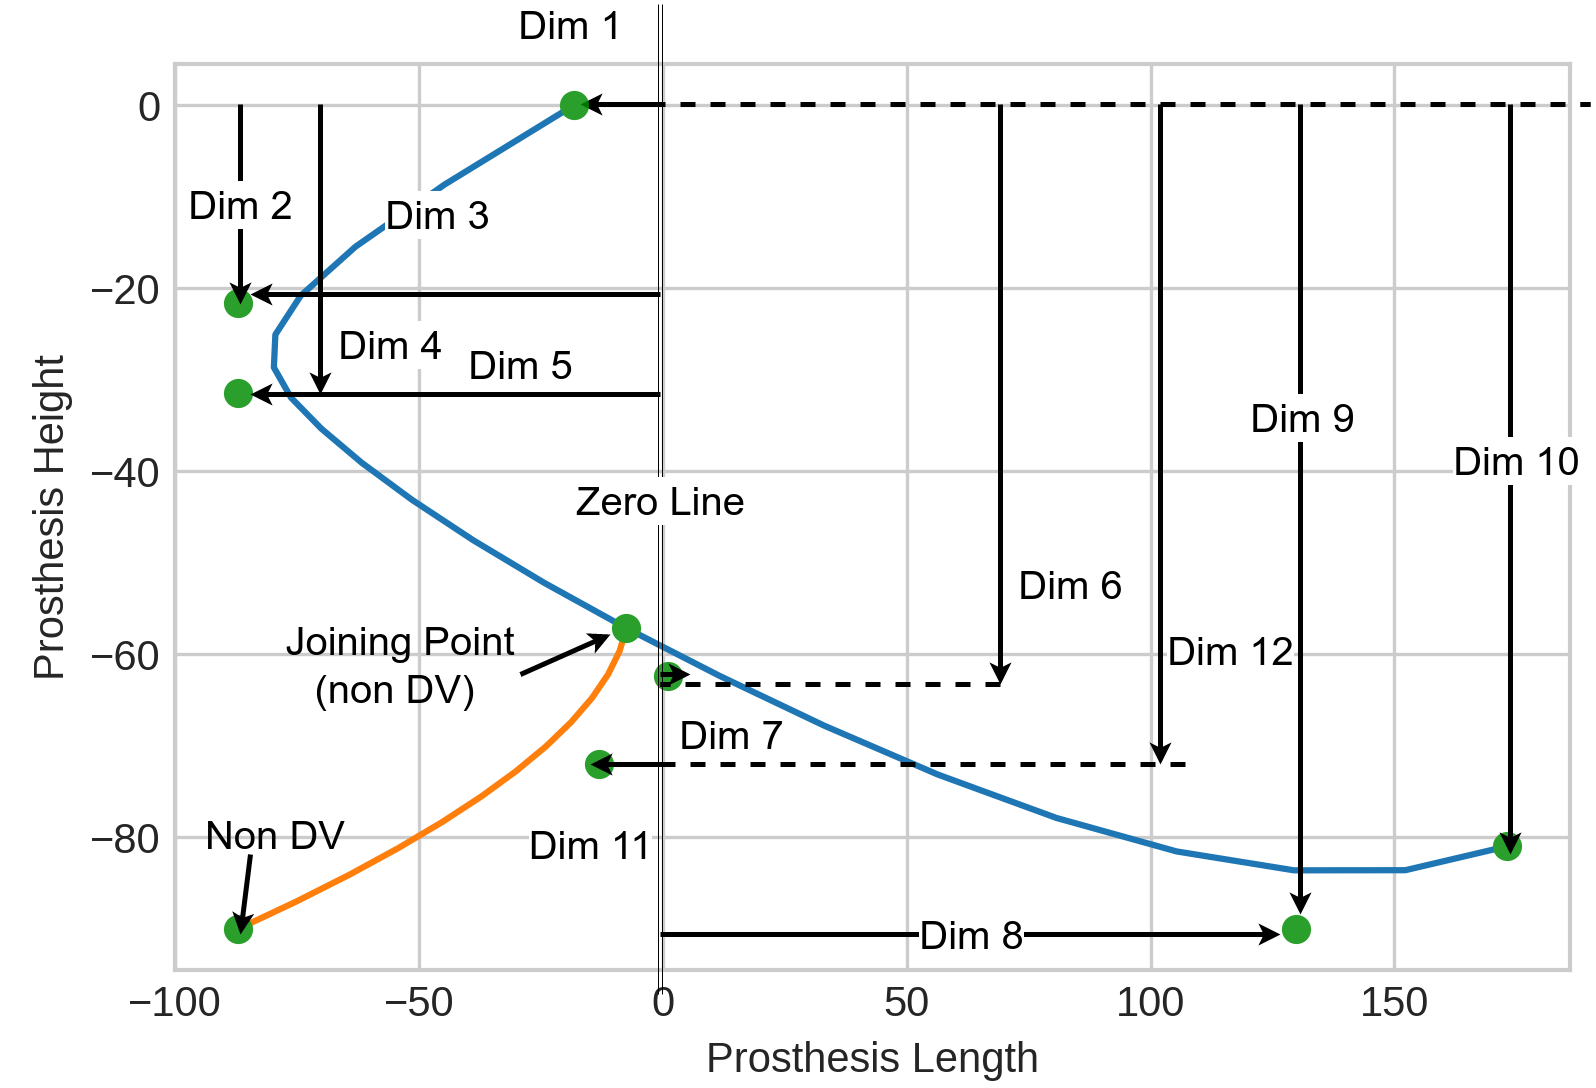
\includegraphics{ShapeDimensionsAF.png}
    \caption{Indicative dimensions for every control point in the Ankle-foot saggital shape. Non DV means: Non Design Variable.}
    \label{fig:shape}
\end{figure}

The respective dimensions of the dimensions mentioned above, are
depicted in the following dataframe:

    \begin{tcolorbox}[breakable, size=fbox, boxrule=1pt, pad at break*=1mm,colback=cellbackground, colframe=cellborder]
\prompt{In}{incolor}{5}{\boxspacing}
\begin{Verbatim}[commandchars=\\\{\}]
\PY{n}{Shape\PYZus{}df} \PY{o}{=} \PY{n}{pd}\PY{o}{.}\PY{n}{read\PYZus{}csv}\PY{p}{(}\PY{l+s+s1}{\PYZsq{}}\PY{l+s+s1}{AnkleFoot\PYZus{}shape.csv}\PY{l+s+s1}{\PYZsq{}}\PY{p}{,} \PY{n}{index\PYZus{}col}\PY{o}{=}\PY{l+m+mi}{0}\PY{p}{)}
\PY{n}{Shape\PYZus{}df}\PY{o}{.}\PY{n}{index} \PY{o}{=} \PY{n}{Shape\PYZus{}df}\PY{p}{[}\PY{l+s+s1}{\PYZsq{}}\PY{l+s+s1}{Experiment No.}\PY{l+s+s1}{\PYZsq{}}\PY{p}{]}\PY{o}{.}\PY{n}{astype}\PY{p}{(}\PY{l+s+s1}{\PYZsq{}}\PY{l+s+s1}{int64}\PY{l+s+s1}{\PYZsq{}}\PY{p}{)} \PY{c+c1}{\PYZsh{}Establiching index experiment}
\PY{n}{Shape\PYZus{}df} \PY{o}{=}  \PY{n}{Shape\PYZus{}df}\PY{o}{.}\PY{n}{drop}\PY{p}{(}\PY{p}{[}\PY{l+s+s1}{\PYZsq{}}\PY{l+s+s1}{Experiment No.}\PY{l+s+s1}{\PYZsq{}}\PY{p}{]}\PY{p}{,} \PY{n}{axis}\PY{o}{=}\PY{l+m+mi}{1}\PY{p}{)} \PY{c+c1}{\PYZsh{}Dropping index column}
\PY{n}{Shape\PYZus{}df}\PY{o}{.}\PY{n}{head}\PY{p}{(}\PY{p}{)}\PY{o}{.}\PY{n}{iloc}\PY{p}{[}\PY{p}{:}\PY{p}{,}\PY{p}{:}\PY{l+m+mi}{12}\PY{p}{]}
\end{Verbatim}
\end{tcolorbox}

            \begin{tcolorbox}[breakable, size=fbox, boxrule=.5pt, pad at break*=1mm, opacityfill=0]
\prompt{Out}{outcolor}{5}{\boxspacing}
\begin{Verbatim}[commandchars=\\\{\}]
                dim 1  dim 2  dim 3  dim 4  dim 5  dim 6  dim 7  dim 8  dim 9  \textbackslash{}
Experiment No.
1               0.738  1.987  0.119  1.762  0.590  48.25  0.148  0.625  1.079
2               0.862  1.979  0.461  1.142  0.230 -55.25  0.988  0.886  0.989
3               0.388  0.824  0.449  1.630  0.874  -7.55  0.742  0.764  0.946
4               0.788  2.181  0.399  1.398  0.966  31.15  0.587  0.627  0.981
5               0.162  2.134  0.491  1.181  0.902  14.95  0.872  0.672  0.789

                dim 10  dim 11  dim 12
Experiment No.
1                0.942   1.136   0.753
2                0.609   1.286   0.948
3                0.796   1.489   0.963
4                0.862   1.016   0.854
5                1.041   1.271   0.992
\end{Verbatim}
\end{tcolorbox}
        
    In order to maintain the proportion, most of the prosthesis preserve
25\% of the shape to the left of the zero line (being this straight to
the tibia position) and the distal point may be positioned up to 75\% of
the total length. Hence, dimensions 1, 3, 5 and 11 are measured
proportionally with respect to the maximum left size, which means 25\%
of the total length. In other words, if dim 1 is 0.738 and the total
length of the foot is 250 mm, the position of this point in \(x\) will
be \(0.738\times-0.25\times250mm = -46mm\)

Similarly, dimension 8 will be evaluated with respect to the remaining
75\% right proportion, whereas for dimensions 2, 4, 9, 12 and 10 will be
the proportion of the max height of the foot, it means: dimension 9 is
1.079 for a 130 mm prosthesis height, in milimeters is translated to:
\(1.079 \times 130mm = 140.27mm\).

Varying those points can give us many design shapes, as shown in Fig.
\ref{fig:many_shapes}.

\begin{figure}[h]
    \centering
    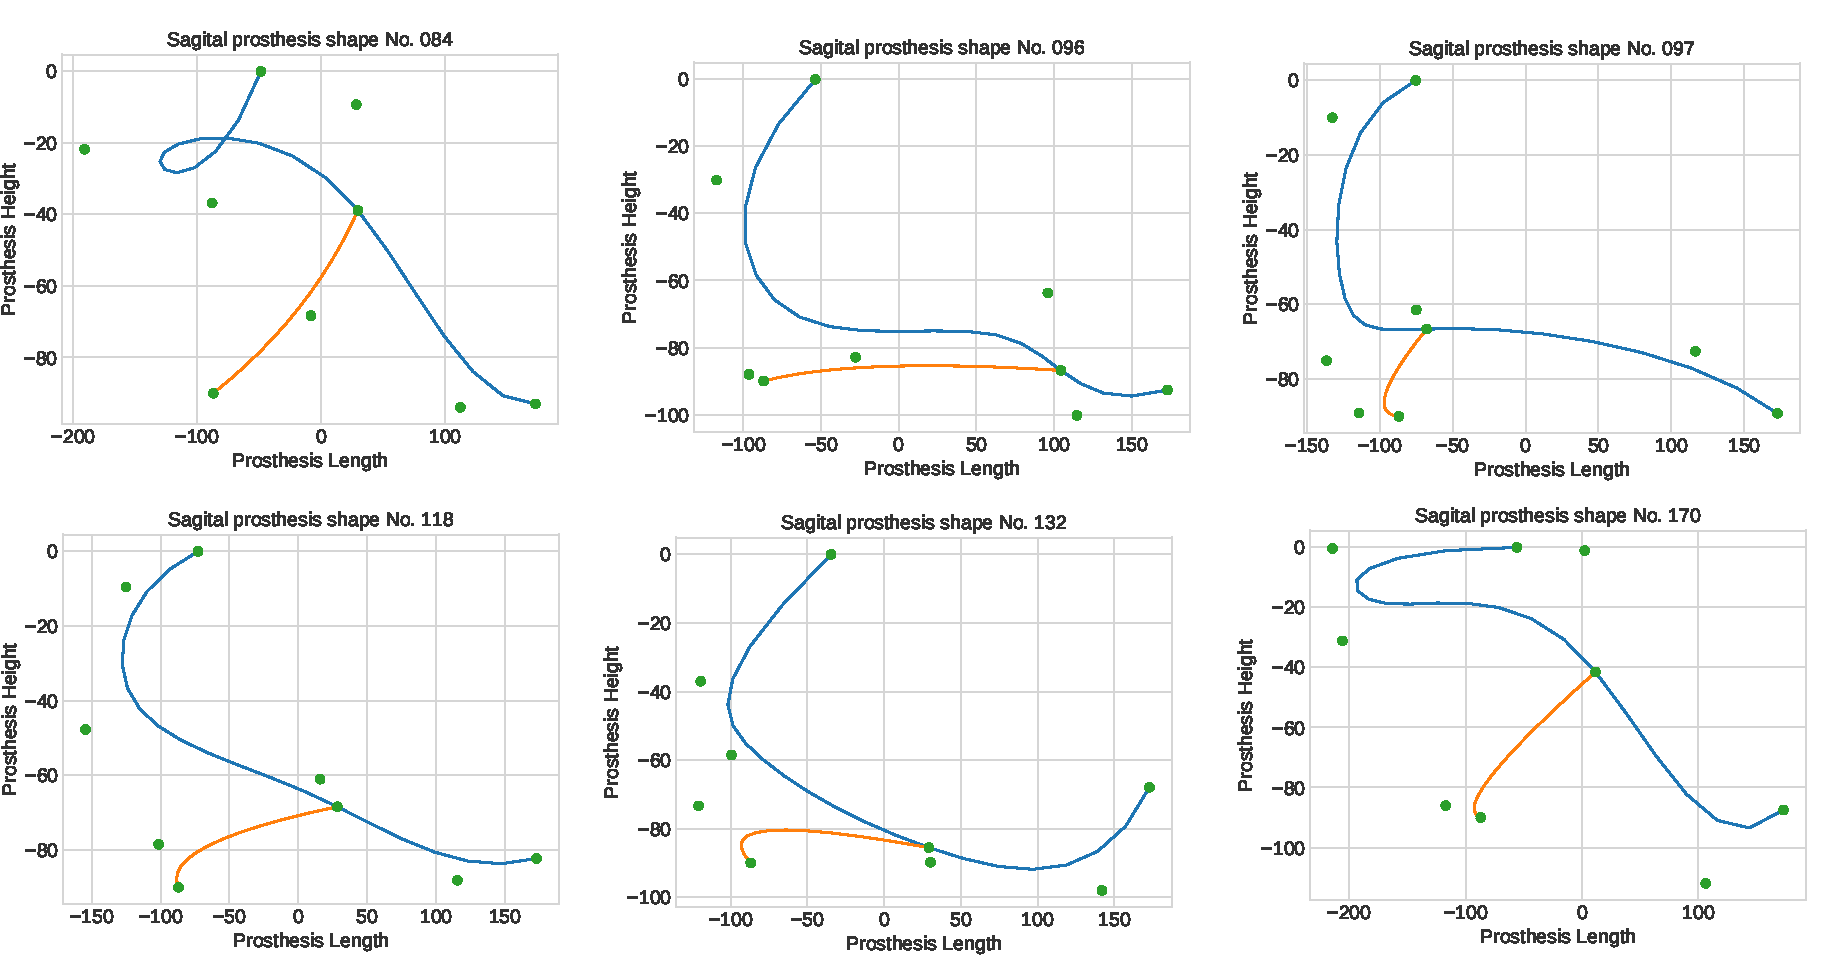
\includegraphics{shapesAF.png}
    \caption{Six randomic designs generated through Latin Hypercupe Sampling.}
    \label{fig:many_shapes}
\end{figure}

The unique point that does not work relative to the foot proportion are
the dims 6 and 7. this point may vary either before or after the zero
line, that is why those points are being controlled in mm.

\hypertarget{outputs}{%
\subsection{Outputs}\label{outputs}}

Either for shape or thickness design, the outputs are the same in both
dataframes. First of all, in the dynamic process you will need to know
how much stress is exerted in the prosthesis, this is an important
variable that cannot exceed the yield stress of the material. Also,
these laminates are composite materials, they are exposed to cyclic
loops and the safety for the user must be guaranteed. These variable in
the column \textbf{MPa} in the dataframe. For your design, consider that
you cannot exceed the \(900MPa\)

    \begin{tcolorbox}[breakable, size=fbox, boxrule=1pt, pad at break*=1mm,colback=cellbackground, colframe=cellborder]
\prompt{In}{incolor}{8}{\boxspacing}
\begin{Verbatim}[commandchars=\\\{\}]
\PY{n}{Shape\PYZus{}df}\PY{o}{.}\PY{n}{head}\PY{p}{(}\PY{p}{)}\PY{o}{.}\PY{n}{iloc}\PY{p}{[}\PY{p}{:}\PY{p}{,}\PY{l+m+mi}{12}\PY{p}{:}\PY{p}{]}
\end{Verbatim}
\end{tcolorbox}

            \begin{tcolorbox}[breakable, size=fbox, boxrule=.5pt, pad at break*=1mm, opacityfill=0]
\prompt{Out}{outcolor}{8}{\boxspacing}
\begin{Verbatim}[commandchars=\\\{\}]
                     MPa  Error\_GRF   MechWork  ErrorMom        RoM
Experiment No.
1               639.5904   0.035172   0.002248  2.442129   2.542826
2               678.8516   0.015182   0.015457  1.480014  19.319449
3               697.6824   0.017248   8.633470  1.303972  27.260984
4               617.7568   0.037799   7.744428  2.079074  26.291950
5               698.1921   0.044156  14.864731  1.539913  31.093966
\end{Verbatim}
\end{tcolorbox}
        
    \hypertarget{error-in-the-grf-and-moment-trajectory}{%
\subsubsection{Error in the GRF and Moment
trajectory}\label{error-in-the-grf-and-moment-trajectory}}

As you see in the data, there are two columns with names
\textbf{Error\_GRF} and \textbf{ErrorMom}. Those are the Mean Square
Error (MSE) measurements for the Ground Reaction Force (GRF) and dynamic
moment trajectory, respectively.

\begin{itemize}
\tightlist
\item
  GRF Error.
\end{itemize}

They were measured through reading raw data on each simulation. The
desired output is the blue one. For the raw data we have applied a
butterworth filter in order to smooth the real output and measure the
error through the minimum Mean Square Error. See Fig \ref{fig:GRF}
for more details

\begin{figure}[H]
\centerline{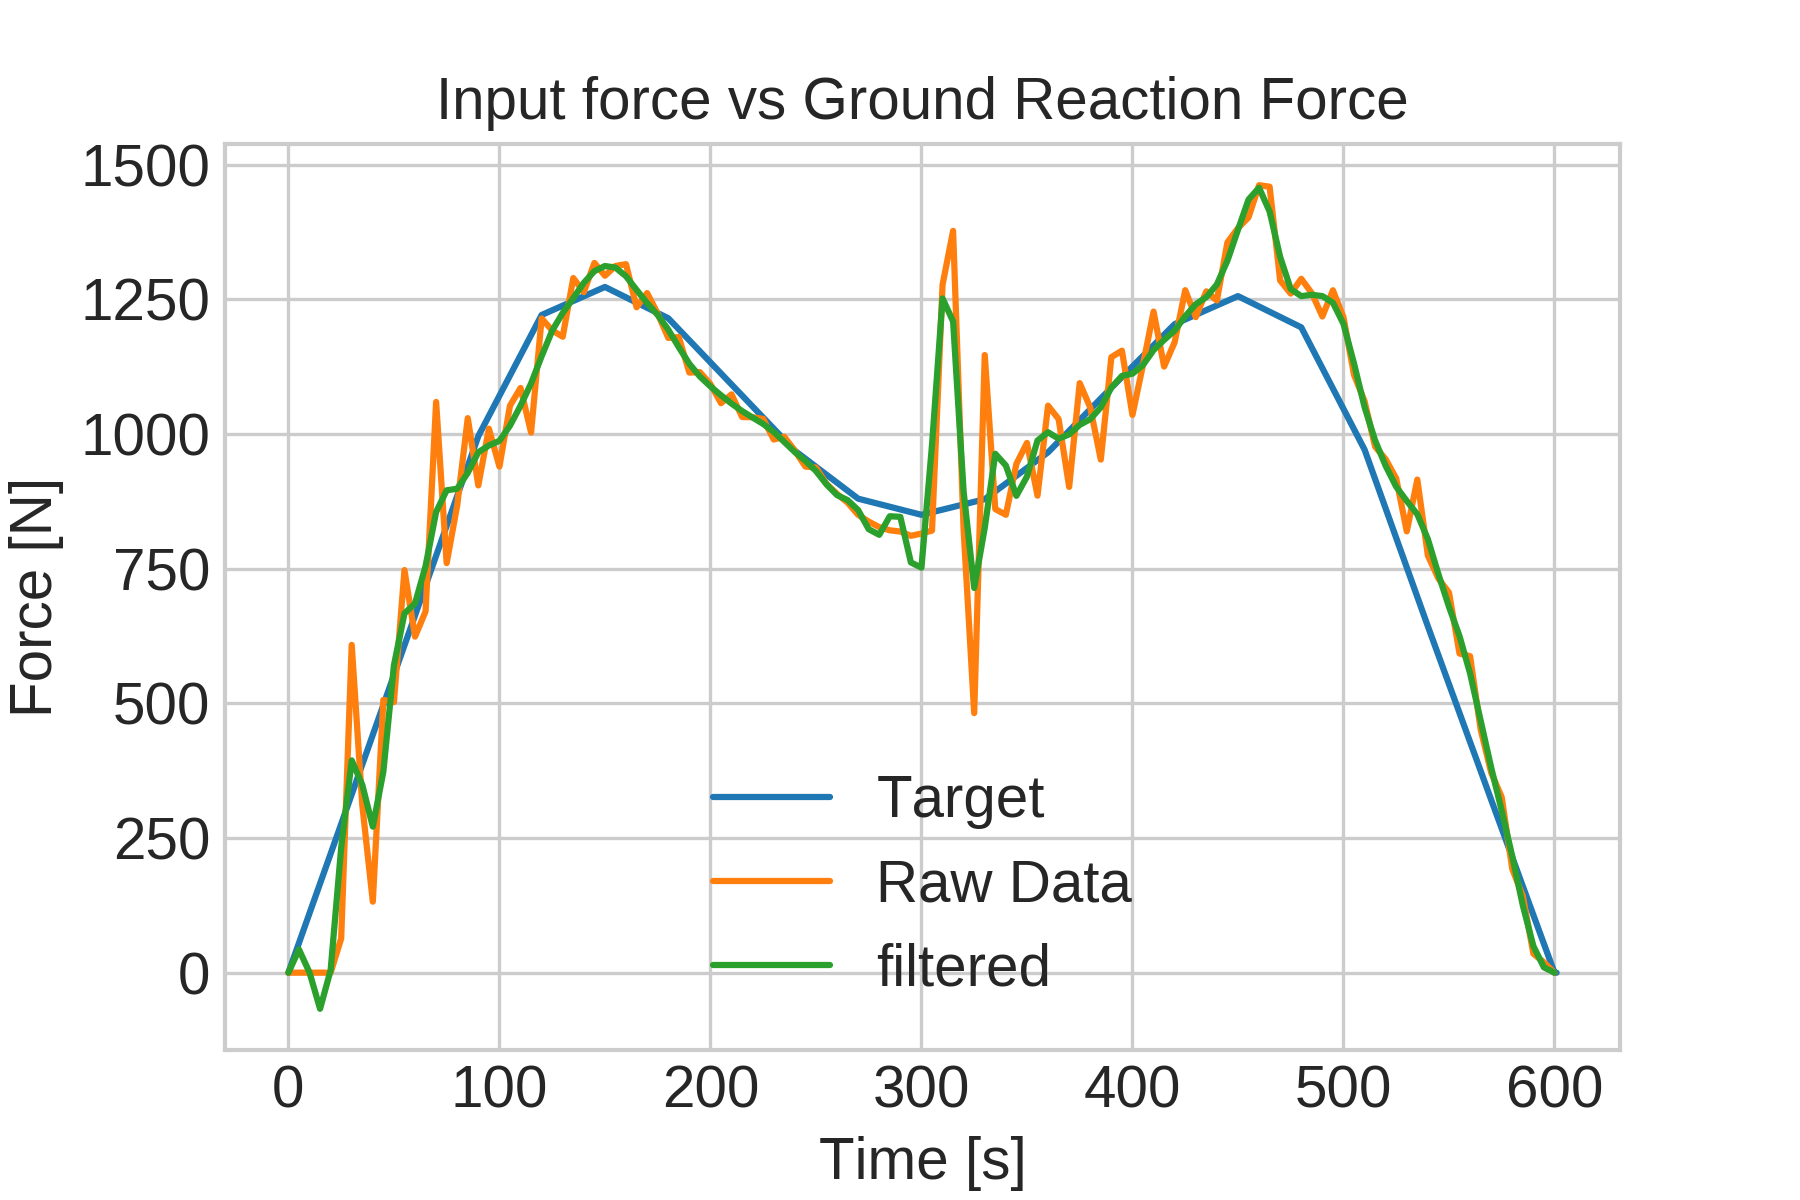
\includegraphics{ErrorGRF.png}}
\caption{\label{fig:GRF} Ground Reaction Forces trajectories in one sample, representing the target as blue color, the pure data (orange) and the filtered results (green) are the outputs of the simulations.}
\end{figure}

\begin{itemize}
\tightlist
\item
  Errors in moments.
\end{itemize}

One of the most important outputs is the torque generated in the ankle
joint. The main purpose is to replicate a natural ankle dynamics with
the prosthesis thus we are comparing the torque generated in the
prosthesis (blue) with a target (green line). therefore, we also have
measured the MSE between both functions, see Fig. \ref{fig:Mom_error}.

\begin{figure}[H]
\centerline{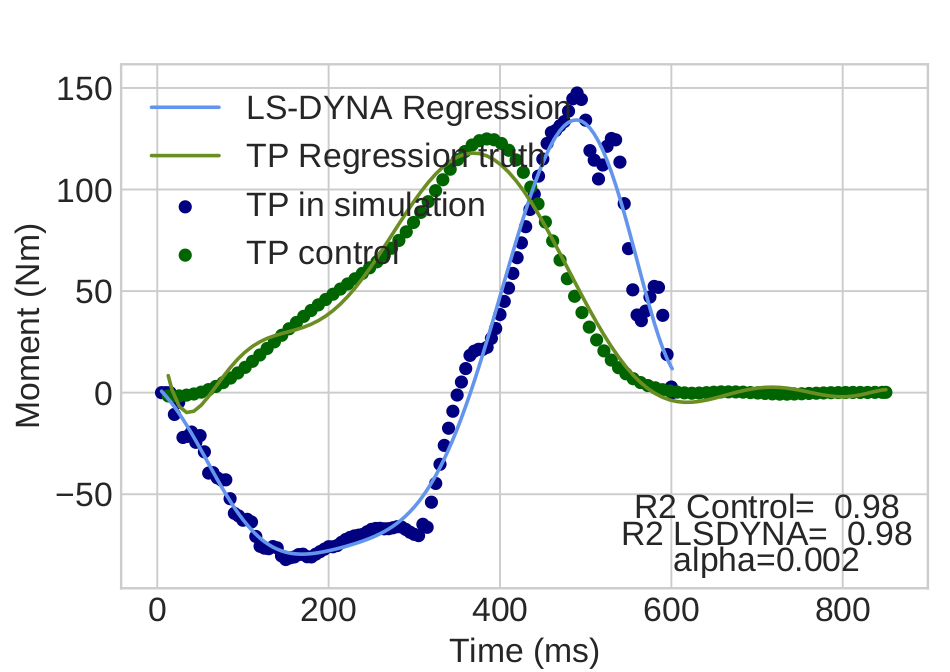
\includegraphics{ErrorMom.png}}
\caption{\label{fig:Mom_error} Regression lines of the moment generated (blue) vs a torque dynamic reference.}
\end{figure}

\hypertarget{range-of-motion}{%
\subsubsection{Range of Motion}\label{range-of-motion}}

Another important feature is to see how compliant is the prosthesis,
this is measured through the Range of Motion (RoM), which is obtained
through the maximum amplitude in the angle dynamic behavior, as shown in
Fig \ref{fig:angle_RoM}, the units are degrees.

\begin{figure}[H]
\centerline{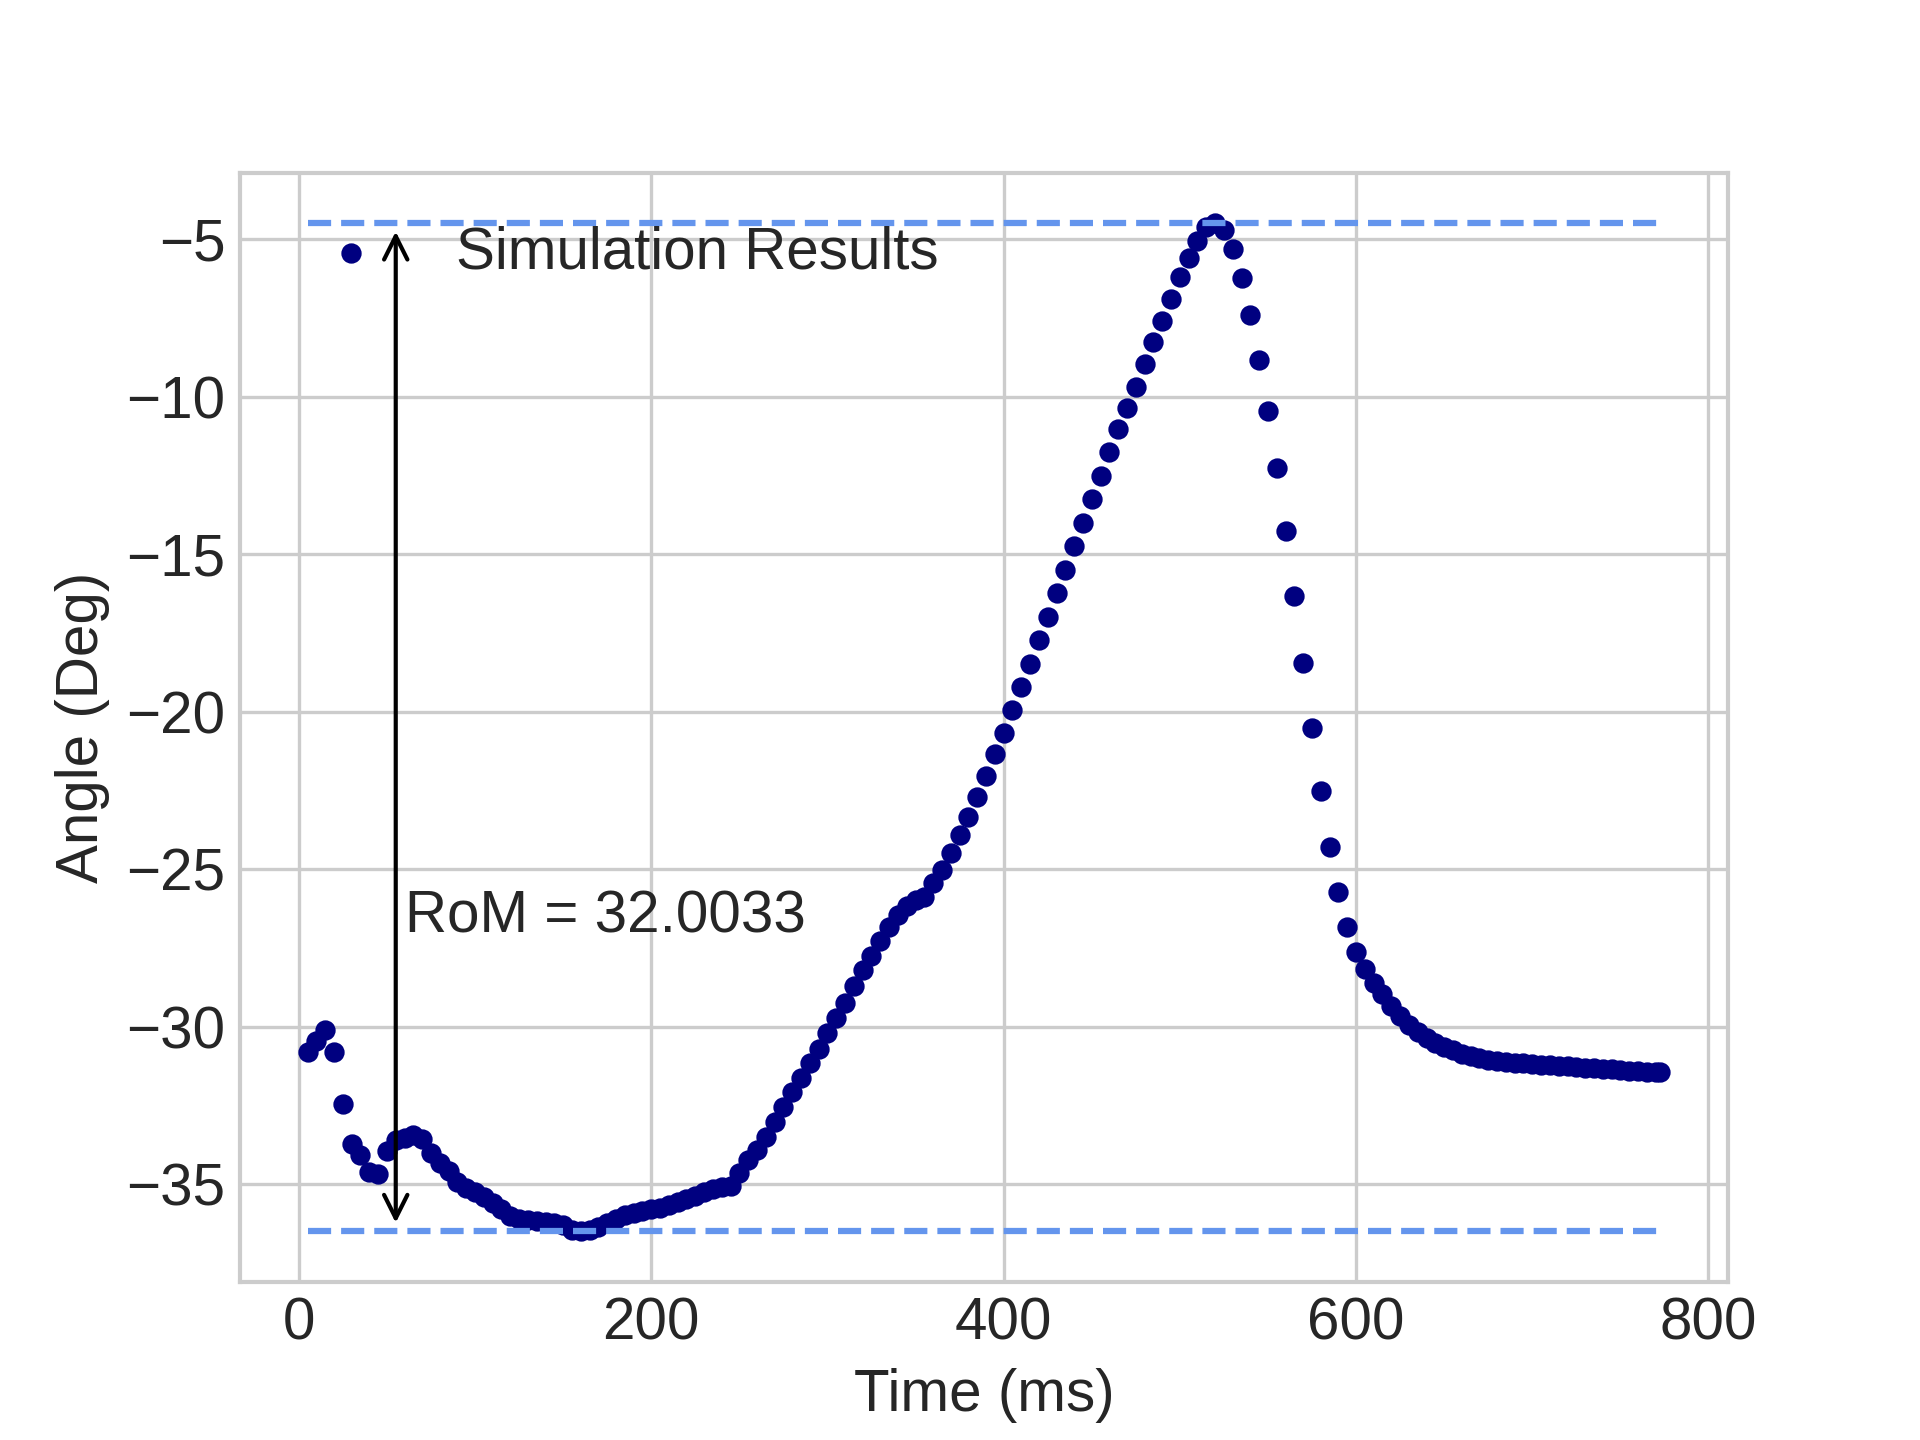
\includegraphics{angle_RoM.png}}
\caption{\label{fig:angle_RoM} Range of Motion measured in ankle-foot prosthesis.}
\end{figure}

\hypertarget{mechanical-work}{%
\subsubsection{Mechanical work}\label{mechanical-work}}

The remaining output is the mechanical work, this is obtained through
the loop integral of the moment respect to the angle. In other words, is
the area of the closed loop of the moment-angle plot. See Fig
\ref{fig:MechWork}.

\begin{figure}[H]
\centerline{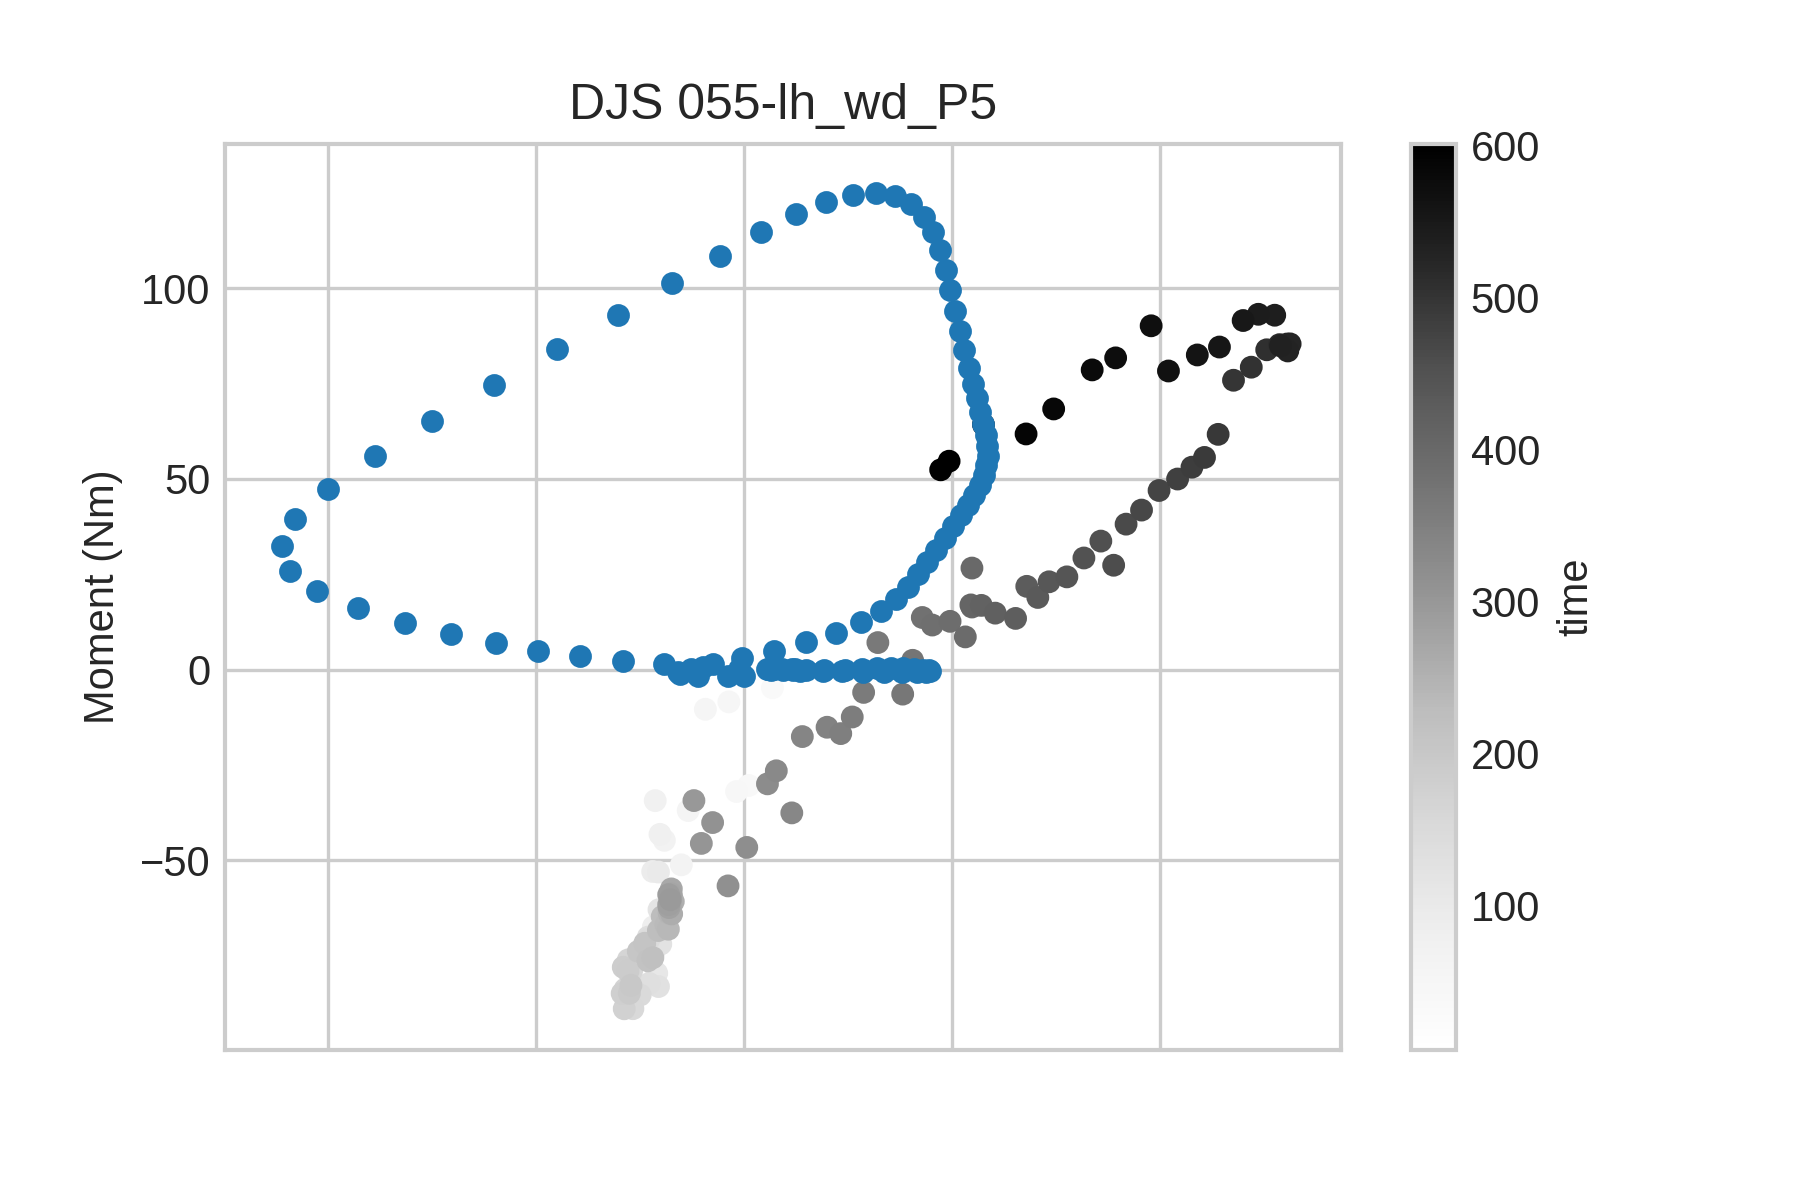
\includegraphics{QS.png}}
\caption{\label{fig:MechWork} Angle-Moment plot of a normal subject (blue dots) vs a prosthesis angle-moment shape. The Mechanical work is obtained through the integral of close loop of those trajectories.}
\end{figure}

    \hypertarget{data-analysis}{%
\subsection{Data analysis}\label{data-analysis}}

As you can percieve in the dataset, this is a multi-label regression
problem. Then, on each output you may apply a regression algorithm to
fit the data and predict another future value. The following is an
example using random forest for only one output in the shape design
dataframe:

    \begin{tcolorbox}[breakable, size=fbox, boxrule=1pt, pad at break*=1mm,colback=cellbackground, colframe=cellborder]
\prompt{In}{incolor}{12}{\boxspacing}
\begin{Verbatim}[commandchars=\\\{\}]
\PY{k+kn}{import} \PY{n+nn}{numpy} \PY{k}{as} \PY{n+nn}{np}
\PY{k+kn}{from} \PY{n+nn}{sklearn}\PY{n+nn}{.}\PY{n+nn}{model\PYZus{}selection} \PY{k+kn}{import} \PY{n}{train\PYZus{}test\PYZus{}split}
\PY{k+kn}{from} \PY{n+nn}{sklearn}\PY{n+nn}{.}\PY{n+nn}{model\PYZus{}selection} \PY{k+kn}{import} \PY{n}{RandomizedSearchCV}
\PY{k+kn}{from} \PY{n+nn}{sklearn}\PY{n+nn}{.}\PY{n+nn}{ensemble} \PY{k+kn}{import} \PY{n}{RandomForestRegressor}

\PY{c+c1}{\PYZsh{}Only for Von misses stress}
\PY{n}{X\PYZus{}train}\PY{p}{,} \PY{n}{X\PYZus{}test}\PY{p}{,} \PY{n}{Y\PYZus{}train}\PY{p}{,} \PY{n}{Y\PYZus{}test} \PY{o}{=} \PY{n}{train\PYZus{}test\PYZus{}split}\PY{p}{(}\PY{n}{Shape\PYZus{}df}\PY{o}{.}\PY{n}{iloc}\PY{p}{[}\PY{p}{:}\PY{p}{,}\PY{p}{:}\PY{l+m+mi}{12}\PY{p}{]}\PY{p}{,} 
                                                    \PY{n}{Shape\PYZus{}df}\PY{o}{.}\PY{n}{loc}\PY{p}{[}\PY{p}{:}\PY{p}{,}\PY{l+s+s1}{\PYZsq{}}\PY{l+s+s1}{MPa}\PY{l+s+s1}{\PYZsq{}}\PY{p}{]}\PY{p}{,} \PY{n}{test\PYZus{}size}\PY{o}{=}\PY{l+m+mf}{0.2}\PY{p}{)}

\PY{c+c1}{\PYZsh{} Number of trees in random forest}
\PY{n}{n\PYZus{}estimators} \PY{o}{=} \PY{p}{[}\PY{n+nb}{int}\PY{p}{(}\PY{n}{x}\PY{p}{)} \PY{k}{for} \PY{n}{x} \PY{o+ow}{in} \PY{n}{np}\PY{o}{.}\PY{n}{linspace}\PY{p}{(}\PY{n}{start} \PY{o}{=} \PY{l+m+mi}{50}\PY{p}{,} \PY{n}{stop} \PY{o}{=} \PY{l+m+mi}{2000}\PY{p}{,} \PY{n}{num} \PY{o}{=} \PY{l+m+mi}{50}\PY{p}{)}\PY{p}{]}
\PY{c+c1}{\PYZsh{} Number of features to consider at every split}
\PY{n}{max\PYZus{}features} \PY{o}{=} \PY{p}{[}\PY{l+s+s1}{\PYZsq{}}\PY{l+s+s1}{auto}\PY{l+s+s1}{\PYZsq{}}\PY{p}{,} \PY{l+s+s1}{\PYZsq{}}\PY{l+s+s1}{sqrt}\PY{l+s+s1}{\PYZsq{}}\PY{p}{,} \PY{k+kc}{None}\PY{p}{]}
\PY{c+c1}{\PYZsh{} Maximum number of levels in tree}
\PY{n}{max\PYZus{}depth} \PY{o}{=} \PY{p}{[}\PY{n+nb}{int}\PY{p}{(}\PY{n}{x}\PY{p}{)} \PY{k}{for} \PY{n}{x} \PY{o+ow}{in} \PY{n}{np}\PY{o}{.}\PY{n}{linspace}\PY{p}{(}\PY{l+m+mi}{10}\PY{p}{,} \PY{l+m+mi}{200}\PY{p}{,} \PY{n}{num} \PY{o}{=} \PY{l+m+mi}{20}\PY{p}{)}\PY{p}{]}
\PY{n}{max\PYZus{}depth}\PY{o}{.}\PY{n}{append}\PY{p}{(}\PY{k+kc}{None}\PY{p}{)}
\PY{c+c1}{\PYZsh{} Minimum number of samples required to split a node}
\PY{n}{min\PYZus{}samples\PYZus{}split} \PY{o}{=} \PY{p}{[}\PY{l+m+mi}{2}\PY{p}{,} \PY{l+m+mi}{3}\PY{p}{,} \PY{l+m+mi}{4}\PY{p}{,} \PY{l+m+mi}{5}\PY{p}{,} \PY{l+m+mi}{10}\PY{p}{,} \PY{l+m+mi}{20}\PY{p}{]}
\PY{c+c1}{\PYZsh{} Minimum number of samples required at each leaf node}
\PY{n}{min\PYZus{}samples\PYZus{}leaf} \PY{o}{=} \PY{p}{[}\PY{l+m+mi}{1}\PY{p}{,} \PY{l+m+mi}{2}\PY{p}{,} \PY{l+m+mi}{4}\PY{p}{,} \PY{l+m+mi}{8}\PY{p}{]}
\PY{c+c1}{\PYZsh{} Method of selecting samples for training each tree}
\PY{n}{bootstrap} \PY{o}{=} \PY{p}{[}\PY{k+kc}{True}\PY{p}{,} \PY{k+kc}{False}\PY{p}{]}

\PY{c+c1}{\PYZsh{} Creating the random grid}
\PY{n}{random\PYZus{}grid} \PY{o}{=} \PY{p}{\PYZob{}}\PY{l+s+s1}{\PYZsq{}}\PY{l+s+s1}{n\PYZus{}estimators}\PY{l+s+s1}{\PYZsq{}}\PY{p}{:} \PY{n}{n\PYZus{}estimators}\PY{p}{,}
               \PY{l+s+s1}{\PYZsq{}}\PY{l+s+s1}{max\PYZus{}features}\PY{l+s+s1}{\PYZsq{}}\PY{p}{:} \PY{n}{max\PYZus{}features}\PY{p}{,}
               \PY{l+s+s1}{\PYZsq{}}\PY{l+s+s1}{max\PYZus{}depth}\PY{l+s+s1}{\PYZsq{}}\PY{p}{:} \PY{n}{max\PYZus{}depth}\PY{p}{,}
               \PY{l+s+s1}{\PYZsq{}}\PY{l+s+s1}{min\PYZus{}samples\PYZus{}split}\PY{l+s+s1}{\PYZsq{}}\PY{p}{:} \PY{n}{min\PYZus{}samples\PYZus{}split}\PY{p}{,}
               \PY{l+s+s1}{\PYZsq{}}\PY{l+s+s1}{min\PYZus{}samples\PYZus{}leaf}\PY{l+s+s1}{\PYZsq{}}\PY{p}{:} \PY{n}{min\PYZus{}samples\PYZus{}leaf}\PY{p}{,}
               \PY{l+s+s1}{\PYZsq{}}\PY{l+s+s1}{bootstrap}\PY{l+s+s1}{\PYZsq{}}\PY{p}{:} \PY{n}{bootstrap}\PY{p}{\PYZcb{}}
\PY{c+c1}{\PYZsh{} Use the random grid to search for best hyperparameters}
\PY{c+c1}{\PYZsh{} First create the base model to tune}

\PY{n}{rf} \PY{o}{=} \PY{n}{RandomForestRegressor}\PY{p}{(}\PY{n}{random\PYZus{}state} \PY{o}{=} \PY{l+m+mi}{42}\PY{p}{)}
\PY{c+c1}{\PYZsh{} Random search of parameters, using 3 fold cross validation, }
\PY{c+c1}{\PYZsh{} search across 100 different combinations, and use all available cores}
\PY{n}{rf\PYZus{}random} \PY{o}{=} \PY{n}{RandomizedSearchCV}\PY{p}{(}\PY{n}{estimator}\PY{o}{=}\PY{n}{rf}\PY{p}{,} \PY{n}{param\PYZus{}distributions}\PY{o}{=}\PY{n}{random\PYZus{}grid}\PY{p}{,}
                          \PY{n}{n\PYZus{}iter} \PY{o}{=} \PY{l+m+mi}{50}\PY{p}{,} \PY{n}{scoring}\PY{o}{=}\PY{l+s+s1}{\PYZsq{}}\PY{l+s+s1}{neg\PYZus{}mean\PYZus{}absolute\PYZus{}error}\PY{l+s+s1}{\PYZsq{}}\PY{p}{,} 
                          \PY{n}{cv} \PY{o}{=} \PY{l+m+mi}{3}\PY{p}{,} \PY{n}{verbose}\PY{o}{=}\PY{l+m+mi}{1}\PY{p}{,} \PY{n}{random\PYZus{}state}\PY{o}{=}\PY{l+m+mi}{42}\PY{p}{,} \PY{n}{n\PYZus{}jobs}\PY{o}{=}\PY{o}{\PYZhy{}}\PY{l+m+mi}{1}\PY{p}{,}
                          \PY{n}{return\PYZus{}train\PYZus{}score}\PY{o}{=}\PY{k+kc}{True}\PY{p}{)}


\PY{n}{rf\PYZus{}random}\PY{o}{.}\PY{n}{fit}\PY{p}{(}\PY{n}{X\PYZus{}train}\PY{p}{,} \PY{n}{Y\PYZus{}train}\PY{p}{)}

\PY{c+c1}{\PYZsh{}concatenating best params obtained with the accuracy}
\PY{n}{results} \PY{o}{=} \PY{n}{rf\PYZus{}random}\PY{o}{.}\PY{n}{best\PYZus{}params\PYZus{}}
\PY{n}{model} \PY{o}{=} \PY{n}{rf\PYZus{}random}\PY{o}{.}\PY{n}{best\PYZus{}estimator\PYZus{}}
\end{Verbatim}
\end{tcolorbox}

    \begin{Verbatim}[commandchars=\\\{\}]
Fitting 3 folds for each of 50 candidates, totalling 150 fits
    \end{Verbatim}

    \begin{Verbatim}[commandchars=\\\{\}]
[Parallel(n\_jobs=-1)]: Using backend LokyBackend with 8 concurrent workers.
[Parallel(n\_jobs=-1)]: Done  34 tasks      | elapsed:   34.4s
[Parallel(n\_jobs=-1)]: Done 150 out of 150 | elapsed:  1.2min finished
    \end{Verbatim}

    the best model for this output is:

    \begin{tcolorbox}[breakable, size=fbox, boxrule=1pt, pad at break*=1mm,colback=cellbackground, colframe=cellborder]
\prompt{In}{incolor}{13}{\boxspacing}
\begin{Verbatim}[commandchars=\\\{\}]
\PY{n}{model}
\end{Verbatim}
\end{tcolorbox}

            \begin{tcolorbox}[breakable, size=fbox, boxrule=.5pt, pad at break*=1mm, opacityfill=0]
\prompt{Out}{outcolor}{13}{\boxspacing}
\begin{Verbatim}[commandchars=\\\{\}]
RandomForestRegressor(max\_depth=50, max\_features=None, min\_samples\_leaf=2,
                      min\_samples\_split=3, n\_estimators=408, random\_state=42)
\end{Verbatim}
\end{tcolorbox}
        
    \hypertarget{sensitivity-analysis}{%
\subsection{Sensitivity Analysis}\label{sensitivity-analysis}}

One of the important characteristics of the ensemble algorithms is to be
able to measure the importance of the variables, in some cases there are
features that are not relevant to the output. Thus that features (or
column) can be omited in future analysis. These is an example of the
permutation importance with the previuos model:

    \begin{tcolorbox}[breakable, size=fbox, boxrule=1pt, pad at break*=1mm,colback=cellbackground, colframe=cellborder]
\prompt{In}{incolor}{ }{\boxspacing}
\begin{Verbatim}[commandchars=\\\{\}]
\PY{k+kn}{from} \PY{n+nn}{sklearn}\PY{n+nn}{.}\PY{n+nn}{inspection} \PY{k+kn}{import} \PY{n}{permutation\PYZus{}importance}
\PY{n}{model}\PY{o}{.}\PY{n}{fit}\PY{p}{(}\PY{n}{X\PYZus{}train}\PY{p}{,} \PY{n}{Y\PYZus{}train}\PY{p}{)}
\PY{n}{perm} \PY{o}{=} \PY{n}{permutation\PYZus{}importance}\PY{p}{(}\PY{n}{model}\PY{p}{,} \PY{n}{X\PYZus{}train}\PY{p}{,} \PY{n}{Y\PYZus{}train}\PY{p}{,} \PY{n}{n\PYZus{}repeats}\PY{o}{=}\PY{l+m+mi}{10}\PY{p}{,}
                                \PY{n}{random\PYZus{}state}\PY{o}{=}\PY{l+m+mi}{42}\PY{p}{,} \PY{n}{n\PYZus{}jobs}\PY{o}{=}\PY{o}{\PYZhy{}}\PY{l+m+mi}{1}\PY{p}{)}
\end{Verbatim}
\end{tcolorbox}

    The higher the number the most important is, some methods can give
values greater than 1, however most of them vary between 0 and 1.

    \begin{tcolorbox}[breakable, size=fbox, boxrule=1pt, pad at break*=1mm,colback=cellbackground, colframe=cellborder]
\prompt{In}{incolor}{17}{\boxspacing}
\begin{Verbatim}[commandchars=\\\{\}]
\PY{n}{pd}\PY{o}{.}\PY{n}{Series}\PY{p}{(}\PY{n}{perm}\PY{p}{[}\PY{l+s+s1}{\PYZsq{}}\PY{l+s+s1}{importances\PYZus{}mean}\PY{l+s+s1}{\PYZsq{}}\PY{p}{]}\PY{p}{)}
\end{Verbatim}
\end{tcolorbox}

            \begin{tcolorbox}[breakable, size=fbox, boxrule=.5pt, pad at break*=1mm, opacityfill=0]
\prompt{Out}{outcolor}{17}{\boxspacing}
\begin{Verbatim}[commandchars=\\\{\}]
0     0.021687
1     0.028002
2     0.031456
3     0.114980
4     0.037173
5     0.044599
6     0.159323
7     0.021985
8     0.126900
9     0.882708
10    0.025654
11    0.015289
dtype: float64
\end{Verbatim}
\end{tcolorbox}
        
    \hypertarget{objective-design}{%
\subsection{Objective design}\label{objective-design}}

Your goal is to design the best prosthesis as possible with the given
data, building metamodels (ML algorithms) for each output, you are free
to implement whatever algorithm available in the literature (XGBoost,
RF, SVM, etc). in order to choose the best design you must consider the
constrains and goal.

\begin{itemize}
\item
  Constrains:
\item
  The maximum Von Misses stress cannot exceed \(1000 MPa\)
\item
  The Range of Motion should be between 22 and 28 degrees.
\item
  The GRF error should be lower than 0.03.
\item
  Goals:
\item
  The least Moment error as possible.
\item
  The Maximum Mechanical work as possible.
\end{itemize}

\hypertarget{activities}{%
\subsection{Activities}\label{activities}}

This is an individual task, your job is the following: 
\begin{itemize}
\item Perform the best ML algorithm that fits the Test set greater than 0.92. Remind the
advantages and disadvantages of each algorithm. For instance, one
disadvantage of RF is that they cannot predict values greater or lower
than the values implied in the dataset, however they provide good scores
whatever the metric implemented. On the other hand, SVM is able to
predict values higher than the bounds, however scaling the data is
needed to provide coherent results. (40\% of the grade) 
\item Perform Sensitivity analysis procedure: Do this analysis with the following
techniques: \href{https://scikit-learn.org/dev/auto_examples/inspection/plot_permutation_importance.html}{Permutation
importance, feature importance} and one the \href{https://salib.readthedocs.io/en/latest/}{Salib packages}. Compare
the results and give conclusions. (20\% of the grade) 
\item Generate an estrategy for obtaining the best values. For instance, you can set a
\href{https://stackoverflow.com/questions/36013063/what-is-the-purpose-of-meshgrid-in-python-numpy}{meshgrid}
with numpy and predict all possible configurations, later you can filter
the best. After that, compare if you have obtained higher values for the
goals and preserving the constrains. (10\% of the grade) \item 
Provide 5 new samples, I will simulate your dimensions and see how far are from
the predicted answers (10\% of the grade). 
\item Presentation and visualization: Remind that good plots and coherent conslusions makes
your work stronger (20\% of the grade) 
\end{itemize}. 

Regards

    \hypertarget{references}{%
\section{References}\label{references}}

\bibliographystyle{unsrt}
\bibliography{biblio.bib}   
    
    
\end{document}
